%%%%%%%%%%%%%%%%%Epic 4%%%%%%%%%%%%%%%%%%%%%%%%%%%%%%%%%%%%%%%%%%%%%%%%%%%%%%%
\subsection{Wegfindung}

In diesem Kapitel wird die Umsetzung des 4. Epics beschrieben. Ziel dieses Epics ist es, dass aufgrund von einem konfigurierten Graphen der schnellste Weg gefunden werden kann und die Kommunikation zwischen Navigation und Steuerung durchgeführt werden kann.

Das Finden des schnellsten Weg in einem Graphen wurde bereits in PREN 1 im Simulator umgesetzt mit einem Dijkstra Algorithmus. Der Simulator wird innerhalb dieses Epics refactored, damit möglichst viele Teile wiederverwendet werden können.

\subsubsection{Wegfindungssoftware aus Simulator anpassen}
\label{navigation-arch}

Bevor der Simulator refactored wurde, wurde die neue Architektur designed für die Navigation, die auf Grafik TODO REF sichtbar ist.

TODO NAVIGATION ARCH BILD

Dieses Refactoring hilft dabei, dass strukturiert die simulierten Teilen mit den realen Teilen ersetzt werden kann und währenddessen trotzdem sowohl auf einem Raspberry Pi, mit allen Verbindungen, als auch auf einem Laptop mit keinen Verbindungen eine lauffähige Version des Simulators verfügbar ist.
Durch verschiedene Environment Variablen\footnote{\url{https://de.wikipedia.org/wiki/Umgebungsvariable}} kann die Hardware und den Funktionsumfang dynamisch gewählt werden. Nachfolgend in Tabelle \ref{table:environment-variables} sind diese Variablen ersichtlich


\begin{table}[H]
    \centering
    \begin{tabularx}{\textwidth}{|X|X|X|}
    \hline
        \textbf{Environment Variable} & \textbf{Beschreibung} & \textbf{Mögliche Werte}\\
        \hline
         \verb|PREN_PLATFORM| & Die Platform, auf welchem der Code ausgeführt wird. & \verb|PC| oder \verb|RPI| \\
         \hline
         \verb|PREN_CAMERA| & Die verwendete Kamera & \verb|NONE|, \verb|USB| oder \verb|PICAMERA| \\
         \hline
         \verb|PREN_UART| & Die verwendete Serielle Schnittstelle für die Kommunikation zwischen Raspberry Pi und TinyK22 & \verb|NONE| oder \verb|<DEVICE>| \newline (z.B. \verb|/dev/ttyAMA0|) \\
         \hline
         \verb|PREN_DISPLAY| & Das verwendete Display &  \verb|NONE|, \verb|OLED| oder \verb|TERMINAL|  \\
         \hline
    \end{tabularx}
    \caption{Environment Variabeln}
    \label{table:environment-variables}
\end{table}

Bei jedem Update wird getestet, ob die Version noch auf allen Plattformen lauffähig ist. Falls dies nicht der Fall wäre, kann durch die Benutzung von Git einfach auf eine alte Version zurück gewechselt werden. So muss das Risiko 14 von Software Updates, die Fehler mit sich bringen, nicht mehr beachtet werden.


Ein grosser Unterschied von dieser Architektur zu der Architektur des Simulators ist es, dass es eine klare Unterteilung in die einzelnen Module gibt, die die Navigation benötigt, so wird paralleles Arbeiten einfacher. Die Architektur modelliert nicht mehr die physischen Roboterteile, sondern nur noch die Navigationsteile.

Der gesamte Sourcecode zu der Navigation kann in folgendem Repository oder im elektronischen Anhang gefunden werden: \url{https://github.com/ameyer3/hslu-pren-navigation}.

Wie im Simulator aus \acrshort{pren1}, wird in der Navigation nach wie vor ein Trial \& Error Modus implementiert. Dieser Modus wird Blind Testing Mode genannt und wird eingeschaltet, falls es wirkt, als ob der Roboter nicht mehr weiss wo er sich befindet, beziehungsweise, falls er denkt er befindet sich auf einem anderen Knoten als er es tatsaechlich tut. Die folgenden Situationen sind Zeichen, dass dies der Fall ist:

\begin{itemize}
    \item Roboter detektiert mehr ausgehenden Kanten von einem Knoten als erwartet.
    \item Falls in einem Winkelbereich, indem keine oder eine Kante erkannt werden soll, zwei Kanten erkannt werden.
    \item Falls der Dijkstra Algorithmus keine Route zum Ziel mehr findet.
\end{itemize}

Im Blind Testing Mode nimmt der Roboter jedes Mal die erste Kante von links, bei der keine Pylone erkannt wird und sucht so das Ziel. Obwohl es noch immer moeglich ist, dass falsche Kanten entfernt werden und dies nicht auffaellt, wird dies akzeptiert. Falls immer noch ein Weg gefunden kann, wird dieser zwar laenger dauern, dies wird aber in Kauf genommen. Mit diesem Konzept koennen Risiko 20 (Roboter weiss nicht mehr wo er sich befindet) und Risiko 7 (Hindernis wird faelschlicherweise erkannt) so stark mitigiert, dass sie vernachlaessigt werden koennen.

\subsubsection{Schnittstelle Navigation und Steuerung}
\label{interface-nav-control}
Die Navigation läuft auf einem Raspberry Pi und die Steuerung läuft auf einem Tiny K22. Die beiden kommunizieren wie geplant über das UART Protokoll miteinander. Für die Kommunikation wurde eine Schnittstelle definiert. Die Navigation sendet 4 Bytes an die Steuerung und die Steuerung antwortet mit dem Statuscode in Form von einem Byte.

Die Instruktionen von der Navigation an die Steuerung, werden, wie in Grafik \ref{fig:interface-tiny} gezeigt, gesendet.

\begin{figure}[H]
\centering
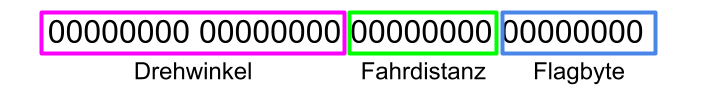
\includegraphics[width=\textwidth]{assets/IT/interface-tiny.png}
\caption{Aufbau Interface zu Steuerung}
\label{fig:interface-tiny}
\end{figure}

Die einzelnen Bytes sind in der folgenden Tabelle \ref{table:interface-to-tiny} beschrieben.

\begin{table}[H]
\centering
\small
\begin{tabularx}{\textwidth}{|c|c|X|}
\hline
  \textbf{Byte} &\textbf{Bezeichnung} & \textbf{Beschreibung}\\
  \hline
      1. Byte&1. Winkelbyte &Zeigt zusammen mit dem 2. Winkelbyte den Drehwinkel an. Die Steuerung addiert die beiden Werte und gibt den Befehl, dass der Robote sich so weit drehen soll. In zwei Bytes aufgeteilt, da Drehwinkel 255 übersteigen kann.\\
  \hline
2. Byte&2. Winkelbyte&Siehe 1. Winkelbyte.\\
  \hline
  3. Byte&Fahrbyte&Gibt die Distanz in Zentimeter an, die der Roboter fahren soll.\\
  \hline
  4. Byte&Flagbyte&Gibt an, ob der Roboter sich nach links oder rechts drehen soll, ob der Roboter vorwärts oder rückwärts fahren soll, ob sich eine Barriere auf der folgenden Strecke befindet.\\
  \hline
  \end{tabularx}
\caption{Interface zu Steurung}
\label{table:interface-to-tiny}
\end{table}

Die einzelnen Bedeutungen zu den Möglichkeiten des Flagbytes sind in Tabelle \ref{table:flag-to-tiny} erklärt.

\begin{table}[H]
\centering
\small
\begin{tabularx}{\textwidth}{|c|X|X|}
\hline
  \textbf{Flagbyte} & \textbf{Bedingung} & \textbf{Beschreibung}\\
  \hline
      0000&nur Winkelbyte gesetzt&Roboter soll sich nach links drehen.\\
  \hline
        0000&nur Fahrbyte gesetzt&Roboter soll vorwärts fahren.\\
  \hline
0001&nur Winkelbyte gesetzt&Roboter soll sich nach rechts drehen.\\
  \hline

0010&nur Fahrbyte gesetzt&Roboter soll rückwärts fahren.\\
  \hline

0100&kein zusätzliches Byte gesetzt&Auf folgender Strecke befindet sich eine Barriere.\\
  \hline
1000&kein zusätzliches Byte gesetzt&Roboter fährt bis er sich auf einem Knoten befindet.\\
  \hline
  \end{tabularx}
\caption{Flags in Interface zu Steurung}
\label{table:flag-to-tiny}
\end{table}



Die möglichen Statuscodes von der Steuerung an der Navigation sind in folgender Tabelle \ref{table:statuscodes} aufgelistet.

\begin{table}[H]
\centering
\small
\begin{tabularx}{\textwidth}{|c|l|X|}
\hline
  \textbf{Statusbyte} & \textbf{Encoding} & \textbf{Beschreibung} \\
  \hline
      00000000&SUCCESSFULLY\_DONE&Befehl wurde erfolgreich ausgeführt. \\
  \hline
00000001&UNEXPECTED\_OBJECT\_DETECTED &Ultraschall hat ein Objeckt erkannt, das nicht erwartet wurde. Navigation macht ein Bild und detektiert, um welches Objekt es sich handelt und handelt entsprechend (mitigiert Risiko 12 (wählt falschen Pfad wegen übersehenden Objekten)): Kehrt um, falls Pylone, beseitigt, falls Barriere.\\
  \hline
\end{tabularx}
\caption{Statuscodes von Steuerung}
\label{table:statuscodes}
\end{table}

\textbf{TinyK22 Implementation}

TODO: WIE SCHNITTSTELLE IN TINY IMPLEMENTIERT

Für jedes Empfangene Byte wird auf dem TinyK22 ein Interrupt generiert und anschliessend ausgelesen. Das Byte wird dann in einem Buffer Array zwischengespeichert. Nachdem die festgelegten 4 Bytes angekommen sind werden die im Buffer zwischengespeicherten Bytes in ein Array geschrieben. Aus diesem Array können dann die einzelnen Funktionen die nötigen Daten entnehmen und weiter verwenden.

\textbf{Raspberry Pi Implementation}

Auf dem Raspberry Pi wurde UART aktiviert, damit dieser mit dem Tiny K22 kommunizieren kann.
Für diese Kommunikation wird ein uart\_connector Modul erstellt. Dieses besteht aus des UARTConnector Klasse und der ErrorHandler Klasse, die die statische Methode 'handle\_errors' enthält. Auf folgender Grafik \ref{fig:uart-connector-nav} sind die beiden Klassen im Detail dargestellt in ihrere Beziehung zu den anderen Klassen.

\begin{figure}[H]
\centering
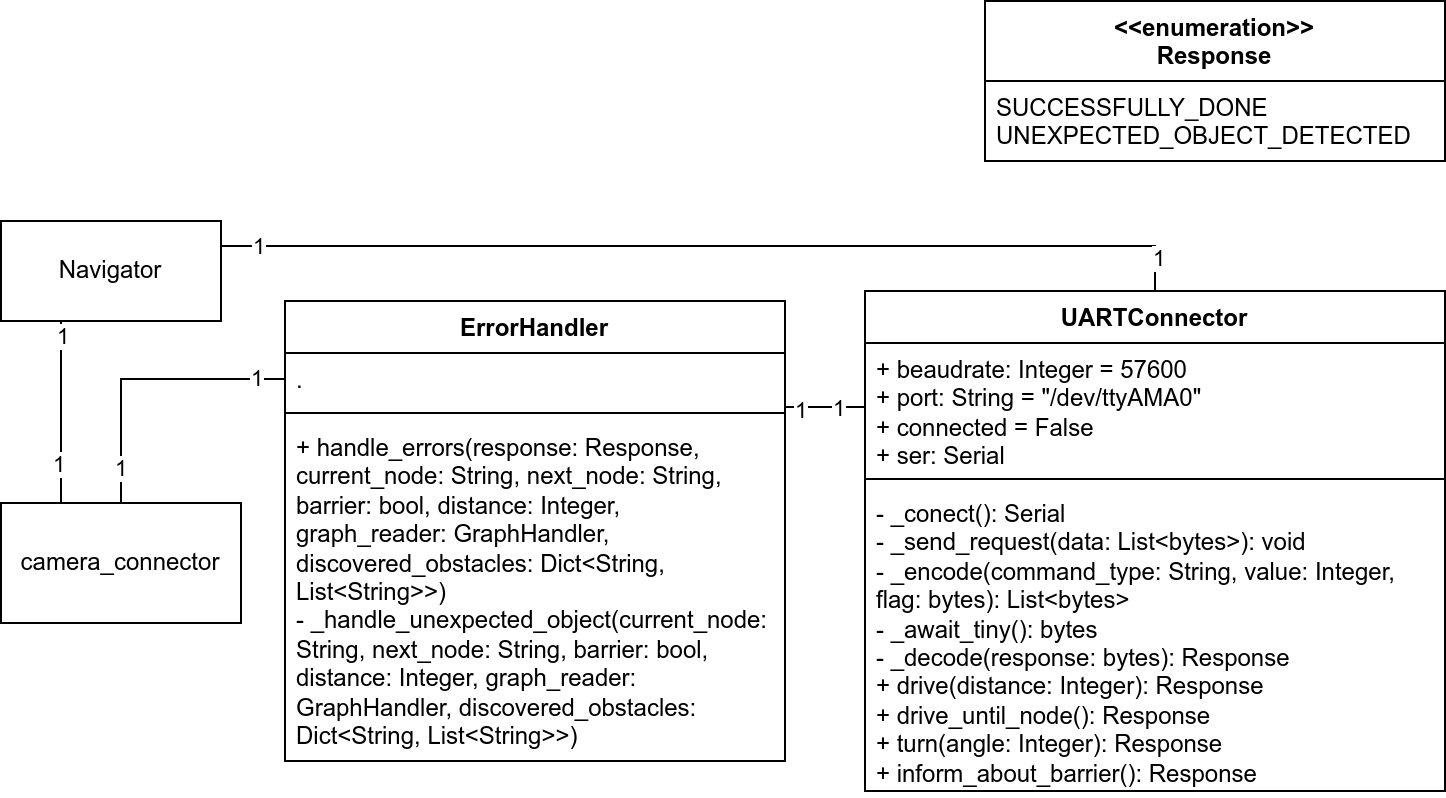
\includegraphics[width=\textwidth]{assets/IT/robot-sw-architecture-uart-connector.png}
\caption{UART Connector und Error Handler Klassendiagramm}
\label{fig:uart-connector-nav}
\end{figure}

Die UART-Connector Klasse  wird mithilfe der PySerial\footnote{https://pypi.org/project/pyserial/} Klasse implementiert. Diese kümmert sich selber um die Start- und Stop-Bits.
Die Verbindung wird mit diesen Zeilen aufgebaut:
\begin{verbatim}
beaudrate = 57600
port = "/dev/ttyAMA0"
self.ser = serial.Serial(self.port, self.beaudrate, timeout=1)
\end{verbatim}

Die Bewegungsinstruktionen werden encoded wie im Interface definiert. Es wird eine Liste mit 4 Bytes erstellt.
Diese Daten werden auf die serielle Verbindung geschrieben.
Danach wird gewartet, bis die Steuerung antwortet. Die Antwort wird wie in Tabelle \ref{table:statuscodes} decoded mit dem Response Enum.
Falls es einen 0 Statuscode (erfolgreich) gibt, wird normal weitergemacht. Falls ein andere Statuscode zurückgegeben wird, wird dieser dem ErrorHandler übergeben.

Der Errorhandler führt die Sequenz aus, die benötigt wird je nach Error.

Das Encoden der Nachrichten wurde mit mehreren Unittests getestet. Diese Unittests, sowie alle folgenden Unittests in der Navigation sind nach dem Muster 'Arrange, Act, Assert'\footnote{https://automationpanda.com/2020/07/07/arrange-act-assert-a-pattern-for-writing-good-tests/} aufgebaut.

Im Arrange Teil wird hier festgelegt, was der Roboter machen soll und wie er antworten soll. Die Antwort wird gemocked\footnote{https://microsoft.github.io/code-with-engineering-playbook/automated-testing/unit-testing/mocking/} mithilfe von der Unittest Library.\footnote{https://docs.python.org/3/library/unittest.mock.html} Beispielsweise soll der Roboter -200cm fahren und die Antwort soll 0 sein, sprich, die Sequenz wurde richtig ausgeführt.

Im Act Teil wird die Funktion aufgerufen, die getest wird. In diesem Beispiel ist das die 'drive' Funktion.

Im Assert Teil wird getestet, ob die zurückgegebene Response korrekt decodiert wurde (von 0 zu SUCESSFULLY\_DONE) und ob die Funktion, die auf den Tiny K22 schreibt, die richtigen Daten gesendet hat, was in diesem Fall ein Array mit folgendem Inhalt wäre:

\begin{verbatim}
# decimal values in Array get converted to Bytes when sent:
# 00000000, 00000000, 11001000 (200 to drive), 00000010 (drive forward)
[0, 0, abs(-200), 2]'
\end{verbatim}

Damit auch ohne Verbindung zu einem Tiny K22 eine lauffähige Version verfügbar ist, wird beim Erstellen der UARTConnector Klasse geprüft, ob eine serielle Verbindung aufgebaut werden konnte. Wenn nicht, werden nach wie vor die alten Teile des Simulators verwendet. Dieser Zustand wird in der 'connected' Variable festgehalten. Dies hilft beim Debuggen und Testen von einzelnen Modulen.


\newpage
%%%%%%%%%%%%%%%%%Epic 5%%%%%%%%%%%%%%%%%%%%%%%%%%%%%%%%%%%%%%%%%%%%%%%%%%%%%%%
\subsection{Hindernis umplatzieren}

Das Umplatzieren eines Hindernisses erfolgt in mehreren Stufen.

\subsubsection{Objekterkennung}
Das Fahrzeug ist mit einem Ultraschallsensor ausgestattet, der zur Detektion von Objekten im Fahrweg eingesetzt werden kann. Die endgültige Entscheidung über das weitere Vorgehen trifft jedoch der \textit{Raspberry Pi}, der mit einer Kamera zur visuellen Objekterkennung verbunden ist.

...... POSSIBLY VERLINKUNG ZU OBJEKTERKENNUNG

Wird ein bewegliches Hindernis erkannt, analysiert das System die Situation. Falls das Hindernis als ausweichbar eingestuft wird, wird ein Wegstellbefehl ausgeführt, um den Fahrweg freizuräumen.

\subsubsection{Wegstellbefehl}
Der \textit{Raspberry Pi} übermittelt dem \textit{TinyK22} einen Drehbefehl sowie einen Befehl zum Rückwärtsfahren, um das Hindernis anzufahren und für das Umplatzieren zu positionieren.

\subsubsection{Bedingung zum Anheben}
Das Fahrzeug fährt rückwärts, bis der Endschalter betätigt wird. Bei Betätigung wird das Fahrzeug gestoppt und der Greifmechanismus

...... POSSIBLY VERLINKUNG ZU Greifmechanismus

aktiviert. Nach dem erfolgreichen Anheben des Objekts dreht sich das Fahrzeug zurück in seine ursprüngliche Ausrichtung. Anschliessend erfolgt eine Nachkorrektur der Position, um das Objekt gezielt wieder abzusetzen.

\subsubsection{Nachkorrektur}
Damit das Hindernis möglichst präzise an der ursprünglichen Position abgelegt werden kann, muss das Fahrzeug seine eigene Position nach korrigieren. Die dafür notwendigen Korrekturwerte wurden experimentell ermittelt.


\newpage
%%%%%%%%%%%%%%%%%Epic 6%%%%%%%%%%%%%%%%%%%%%%%%%%%%%%%%%%%%%%%%%%%%%%%%%%%%%%%
\subsection{Auf Linie ausrichten}

\subsubsection{Roboter drehen}

...NEUE DEFINITION (WIR DREHEN nur noch mit den Liniensensoren, links recht wieder möglich)

...


\subsubsection{Ausgehende Linien erkennen}
\label{outgoing-lines}

...

Falls die ausgehenden Linien nicht erkannt werden können, wird der Roboter 20cm zurueckfahren und in kleinen Abständen vorfahren und Bilder machen und weiterhin versuchen die ausgehenden Kanten zu erkennen. Falls die Linien immer noch nicht erkannt werden koennen, faehrt der Roboter zum letzten Knoten zurueck. entfernt den anderen Knoten aus dem intern gespeicherten Graph und sucht sich einen anderen Weg.